\RequirePackage{plautopatch}
\documentclass[twocolumn,dvipdfmx]{article}
% \usepackage{geometry}
% \geometry{top=0mm}%
% \usepackage[top=0cm,headheight=0pt,headsep=0in,heightrounded]{geometry}
\usepackage{amsmath}
\usepackage{amssymb}
\usepackage{booktabs}
\usepackage{CJK}
\usepackage{courier}
\usepackage{helvet}
\usepackage{latexsym}
\usepackage{marvosym}
\usepackage{multirow}
\usepackage{rotating}
\usepackage{setspace}
\usepackage{stmaryrd}
\usepackage{tabularx}
\usepackage{textcomp}
\usepackage{times}
\usepackage{url}
\usepackage{wasysym}
\usepackage{here}
\usepackage{ascmac}
\usepackage{setspace}
\spacing{0.95}
\usepackage{breakcites}
\usepackage{fancyhdr}
\usepackage{graphicx}

\usepackage{hyperref}
% \usepackage[tracking=true]{microtype}               
% \newcommand\squeeze[1]{\SetTracking{encoding=*}{#1}\lsstyle}
\usepackage{enumitem}
\setlength{\textfloatsep}{0pt plus 0pt minus 0pt}
\setlength{\floatsep}{0pt plus 0pt minus 0pt}
\setlength{\intextsep}{0pt plus 0pt minus 0pt}
\setlength{\dbltextfloatsep}{0pt plus 0pt minus 0pt}
\setlength{\dblfloatsep}{0pt plus 0pt minus 0pt}
\setlength{\abovecaptionskip}{0pt plus 0pt minus 0pt}
\setlength{\belowcaptionskip}{0pt plus 0pt minus 0pt}
\setlength{\itemsep}{0pt plus 0pt minus 0pt}
\setlist[itemize]{noitemsep,topsep=0pt}
\setlist{nolistsep}
\setlist{nosep}
% \usepackage{titlesec}
% \titlespacing{\section}{0pt}
% \titlespacing{\subsection}{0pt}
% \usepackage{biblatex}
\usepackage[compact]{titlesec}
\titlespacing{\section}{1pt}{2ex}{1ex}
\titlespacing{\subsection}{1pt}{1ex}{1ex}
\titlespacing{\subsubsection}{1pt}{1ex}{1ex}
\setlength{\parskip}{0cm}
\setlength{\parindent}{0cm}
% \renewcommand*{\@seccntformat}[1]{\csname the#1\endcsname\hspace{0mm}}


% \renewcommand{\headrulewidth}{1pt}
\fancypagestyle{firstpage}
{
    \fancyhead[L]{}
    \fancyhead[C]{\Large 言語獲得と理解研究会報告(Summer 2024)}    
    \fancyhead[R]{}
}

\setlength{\oddsidemargin}{-3.4mm}
\setlength{\evensidemargin}{-3.4mm}
\setlength{\topmargin}{1.3mm}
\setlength{\headheight}{18pt}
\setlength{\headsep}{-1mm}
\setlength{\textwidth}{18cm}
\setlength{\textheight}{24.4cm}
\setlength{\columnsep}{0.8cm}
\setlength{\leftmargin}{-0.5cm}
\setlength{\itemsep}{0cm}

\baselineskip=0.9\baselineskip
\abovedisplayskip=0.8\abovedisplayskip
\belowdisplayskip=0.8\belowdisplayskip
\abovedisplayshortskip=0.8\abovedisplayshortskip
\belowdisplayshortskip=0.8\belowdisplayshortskip

\renewcommand{\thepage}{}

% \auther{} 
\def\AND{\hskip 2em plus 40fil}

\newcounter{ex}
\newcommand{\itemex}{\refstepcounter{ex}\item[\textmd{\textrm{(\theex)}}]}

\def\ex#1{
\begin{description}
 \itemex #1
\end{description}
}

\title{\textbf{ホテルレビューのデータを用いた感情スコア生成法}}

% \author{
%     First Author \\
%     Affiliation / Address line 1 \\
%     Affiliation / Address line 2 \\
%     Affiliation / Address line 3 \\
%     {\tt email@domain} \\
%     \and
%     Second Author \\
%     Affiliation / Address line 1 \\
%     Affiliation / Address line 2 \\
%     Affiliation / Address line 3 \\
%     {\tt email@domain} \\
%     \and
%     Third Author \\
%     Affiliation / Address line 1 \\
%     Affiliation / Address line 2 \\
%     Affiliation / Address line 3 \\
%     {\tt email@domain} \\
% \date{}\\[-12pt]
% }

%%% OR USE THIS METHOD または著者NOリストを以下のように作成してもよい
% 
% Authors, for the paper (add full first names)
%\Author{Firstname Lastname $^{1,\dagger,\ddagger}$\orcidA{}, Firstname Lastname $^{2,\ddagger}$ and Firstname Lastname $^{2,}$*}
\author{
%\begin{center}
\begin{tabular}{c{1.3in}c{1.3in}c{1.3in}}
        \Large 磯村悠月  \textdagger & \Large シラー ヴィクター  \textdaggerdbl & \Large 高橋海哉 \textdagger \\[6pt]
%\end{tabular}\\[3pt]
\multicolumn{4}{c}{\textdagger\space 
釧路高等工業専門学校 創造工学科 情報分野}\\
\multicolumn{4}{c}{\texttt{p200014@kushiro.kosen-ac.jp}}\\[2pt]
\multicolumn{4}{c}{\textdaggerdbl\space 釧路工業高等専門学校 創造工学科}\\
\multicolumn{4}{c}{\texttt{\{silaa\}@kushiro-ct.ac.jp}}\\
[4pt]
\multicolumn{4}{c}{}\\[-8pt]
\multicolumn{4}{c}{\textbf{Abstract}}\\
%\textbf{Abstract}
\multicolumn{4}{p{6.4in}}{\normalsize
 北海道には様々な観光地が散在して,その観光地のにはレビュー文とともに星の評価がつけられていることが多い.私たちは北海道釧路市において観光地をユーザーに推薦するシステムの構築を検討しているが,ユーザーに観光地を推薦するのならば他のユーザーからの評価は必須である.そのため,ホテルレビューのサンプルデータを用いて自然言語処理でレビューの分類を行い,その分類された精度を用いることでアルゴリズムを評価し,データを分類する際に適切なアルゴリズムを選択できるようにすることが今回の目的である.ホテルレビューの分類においてDistilBERTでも精度が71\%というとても低い結果が得られた.この原因として偏ったデータによる過学習が考えられるが,原因を突き止めてはいない.
}
\end{tabular}
% \end{center}
\date{}\\[-12pt]
}



\begin{document}
% \thispagestyle{firststyle}

\maketitle
% \pagestyle{firstpage}
\thispagestyle{firstpage}
% \thispagestyle{fancy}
% \firstpage{fancy}
% \firstpage{firstpage}

\section{はじめに}
 2024年に国土交通省が行った調査によると,国としての訪日外国人観光客数の推移が2020年度COVID-19感染拡大により観光客数が一気に減っているが,2023年度から回復傾向であり,2024年5月現在に至っては,感染拡大前の5月までの観光客数を越す勢いである.また,北海道の観光入込客数も2022年度から回復しており,観光客数の回復が見込まれる.\cite{hokkaidou_data}

 日本交通公社の「国内旅行におけるSNS,写真に対する意識/実態」によると国内旅行の実施に当たり,各世代の半数がインターネットの検索エンジンを使用し計画を立てている.\cite{baitai_data}そのため観光者数を向上させるためには,インターネット媒体の観光コンテンツのサービス向上を図ることが必要である.

  本研究では,SNSやWebからテキストデータや観光地データなどを収集し,収集したテキストデータを自然言語処理によって分類を行い,ユーザーに対し適切な観光地を推薦させることが目的である.
  
 その第一段階として今回のホテルレビューのデータを様々なアルゴリズムで分類し,得られた精度や時間からアルゴリズムの評価を行うことによって,別の分類を行う際も同様のアルゴリズムを使用して分類を行うことによってより良い精度で分類が行えると考えている.

 なお,今回は観光地のレビュー文をそれぞれの評価別に分類したものを研究結果として扱っている.推薦システムや観光システムは今回は計画段階のものを発表する.



\section{研究背景}
\label{background}
 今回の研究を行った背景としては,今後テキストデータを自然言語処理するにあたり,それぞれのアルゴリズムの特徴を実際に分類を行うことによって知識として持っておきたいという理由と,釧路市は空港こそあるものの交通アクセスが道央圏と比べての悪いのは事実であるため,観光をするにあたって宿泊をしなければならない場合が多いと考えている.そのためホテルのレビューのデータ分類を行うことによってユーザーにより良いホテルを提供したいと考えている.

 また,今後推薦システムを作るにあたって,観光シーズンの分類とレビューの分類,ユーザー情報などの様々な要素によりユーザーに観光地を推薦したいと考えているため,データの分類を行う機会が増えると思うので,今回のアルゴリズムの評価によって使っていくアルゴリズムを決めていきたいと考えている.
  
\section{研究内容}
\label{experiments}
本研究では,観光システムの構築,レビュー文の分類,推薦システムの構築の主に3つの段階があり,今回は観光システムの構築とレビュー文の分類の一部分について研究成果として発表する.

\subsection{観光システムの構築}

 観光地の評価の可視化を行うことでユーザーに対する推薦を行い,観光地を活性化させることが目的であるため,観光システムの構築をすることが必要である.
 
 本研究で構築するシステムは地方の観光地は情報の更新の頻度やレビュー文が少ないという点を鑑みてSNS「X」「Instagram」での情報収集を主に行い,Webでのレビューサイトから観光地情報やレビュー文を収集する.レビュー文の季節の特徴を自然言語処理によって解析し,その特徴やユーザーの情報,観光地情報などの特徴からユーザーにあった観光地を推薦するシステムを構築する.システムの概要図をFigure\ref{system}に示す.

\begin{figure}[htbp]
\begin{center}
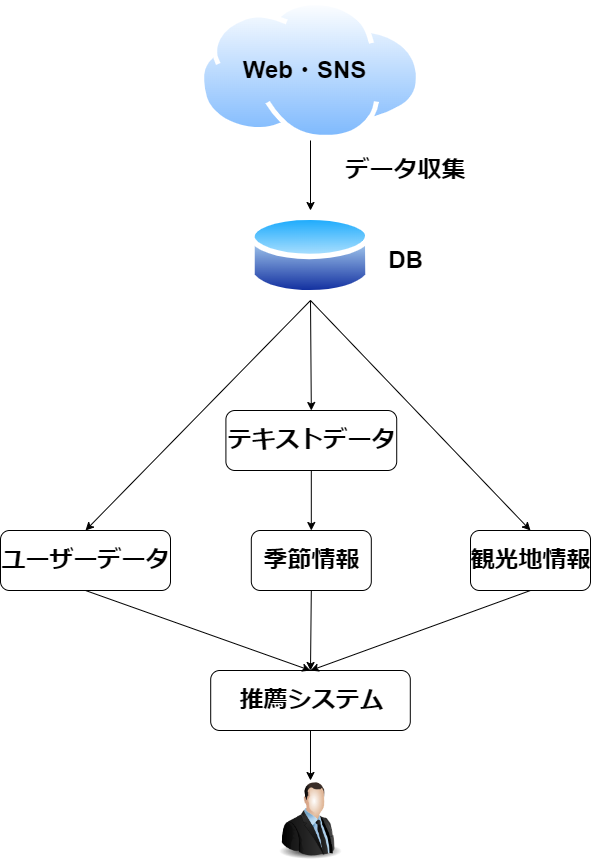
\includegraphics[width=47mm]{system2.png}
\caption{観光システム構成図}
\label{system}
\end{center}
\end{figure}

 このようにしてWebやSNSから収集したデータの中からレビュー文などのテキストデータを自然言語処理を使って分類したものや,ユーザーデータ,観光地情報など複数の情報から協調フィルタリングという推薦システムを用いてユーザーに推薦するシステムを構築したいと考えている.

 













\subsection{レビュー文の分類}

 本研究では株式会社リクルートが提供する"Japanese Realistic Textual Entailment Corpus"\cite{baitai_data}を利用した株式会社リクルートの林部祐太氏が発表した論文\cite{ronbun2}でgood,excellent,badの3種類の評価に分類されたたデータを利用して, Naive Bayes , SVM(Support Vector Machine)  , Decision Tree , Logistic Regression , DistilBERT の5つのモデルアルゴリズムを使って精度を計測し,レビュー文の分類を行うためにどのようなアルゴリズムが最適であるか調べることを目標とした.
 
  レビュー文の総数は5551個あり,それぞれをタイプ別に分けるとFigure\ref{data_type}のようになり,goodが1330件,
 exccelentは3405件,badは818件の数がある.
 
\begin{figure}[htbp]
\begin{center}
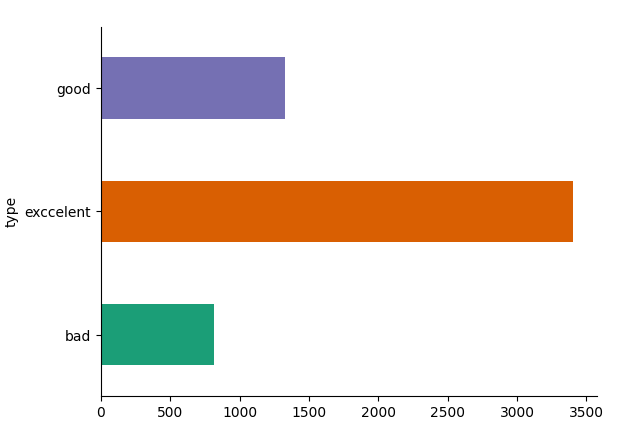
\includegraphics[width=90mm]{data_type.png}
\caption{タイプ別レビュー数}
\label{data_type}
\end{center}
\end{figure}


\begin{table}[htbp]\centering
  \caption{レビュー文のタイプ別内容}
  \label{naiyou}
\begin{tabular}{|l|r|} \hline
  type & レビュー文  \\ \hline
   exccelent & 今回はバタバタでしたが、プライベートで、\\
              &来てもいいと思えるリゾートホテルでした。\\  \hline
   exccelent & とても親切な対応でした。\\  \hline
   good & 出張でお世話になりました。\\   \hline
   good & +:。   \\  \hline
   bad & チェックアウト時も\\    
   &ありがとうございましたもなし。\\ \hline
   bad & 悪かった所:朝食。\\ \hline
 \end{tabular}
\end{table}

また,Figure\ref{naiyou}はホテルのレビュー文を一部抜粋したものである.このように短いレビューから長いレビューまであり,一部スパムのようなレビューも見受けられる.

このようなデータを用いて自然言語処理によってデータをきれいな状態にしてからアルゴリズムを使ってそれぞれの評価を行っていく.
具体的な手順は以下のとおりである.

\begin{enumerate}
  \item レビュー文を読み込む.
  \item レビュー文に対し分かち書きを行い形態素解析器Janomeを使い形態素解析を行う.
  \item 形態素解析を行った後,ストップワードの除去,句読点や無駄な記号を取り除く.
  \item レビュー文を8:2の割合でトレーニング用とテスト用に分ける.
  \item 5つのアルゴリズムを用いてトレーニングとテストを行い精度と実行時間を測る.
\end{enumerate}
 今回の形態素解析器は「Janome」を使用している.理由としてはレビュー文をリストで扱う際に使いやすかったためである.
モデルアルゴリズムでの処理を行う場合,精度を上げるために文章から記号とストップワードを除去しなければならないため,レビュー文に対し分かち書きを行い,形態素解析により単語の品詞を調べ,記号と日本語のストップワードの除去を行った.今回ストップワードの除去で使用した辞書は「slothlib」\cite{slothlib}という辞書から春,夏,秋,冬などの季節を表す語句を除いたものを使用した.


 \subsection{アルゴリズムと分類精度}
  用意した学習データを8:2の割合でトレーニング用とテスト用に分け, Naive Bayes  , SVM , Decision Tree , Logistic Regression , DistilBERT の5つのアルゴリズムでトレーニングおよびテストを行った.
  
 まず,初めに実験に用いた実行環境はFigur\ref{setting}の通りである.
 
\begin{table}[H] \centering
  \caption{実験環境}
  \label{setting}
\begin{tabular}{ll} \hline
 プラットフォーム & Google Colaboratory \\
 コンパイラ & Python3 \\
 GPU & T4 GPU \\ \hline
\end{tabular}
\end{table}
  
 それぞれのアルゴリズムについての解説は以下の通りである.
 
 Naive Bayes は機械学習の教師あり学習に使われる手法であり,ベイズの定理を使い分類するアルゴリズムである.特徴として学習データが膨大でも良く計算時間が速いという特徴がある.\cite{Naivebayse}

 SVMは教師ありの機械学習アルゴリズムであり,高速で信頼性のあるアルゴリズムである.特徴として学習データが少なくてよく過学習も起こしづらいが,学習が非常に非効率であるため,データが膨大になる場合,実行時間が膨大になるという欠点がある.\cite{SVM}
 今回は,コストパラメータを10,RBFカーネルのパラメータを0.1として実験を行った.

 Decision Treeは解釈が容易であり様々なデータをそのまま扱えるのが特徴のアルゴリズムであるが,決して分類性能が高い手法ではなく,過学習を起こしやすいという欠点がある.\cite{Decision Tree}
 
 Logistic Regressionはベルヌーイ分布に従う変数の統計的回帰モデルの一種であり,いくつかの要因から2値の結果が起こる確率を説明・予測することができるアルゴリズムである.
\cite{Logistic Regression}

 BERTとは最近の言語表現モデルとは異なり,全ての層で左右両方の文脈を共同で条件付けることにより、ラベル付けされていないテキストから深い双方向表現を事前に学習するように設計されているものであり,2018年当時の最高精度をたたき出したことで話題となったものである.\cite{BERT}
 DistilBERTは従来のBERTを高性能・高速・軽量化したものであり,BERTの性能を95\%以上維持しながら60\%も高速に動作することが特徴である.\cite{DistilBERT}
 
 今回は,distilbert-base-uncasedというモデルを使い,トレーニングパラメーターとしてEpochsの値は2, Split Ratioは1e-4 としました.また,クラスは3変数, レビューの文字数を最大500, バッチサイズを16として実験を行いました.
 
 
 Table\ref{seido}に各アルゴリズムでのテストスコア及び,トレーニングも含めた実行時間を示す.


\begin{table}[htbp] \centering
  \caption{各アルゴリズムの精度}
  \label{seido}
\begin{tabular}{lrr} \hline
   アルゴリズム & accuracy &  time(s) \\ \hline
   Naive Bayes &  0.33285577 & 0.085806528\\
   SVM & 0.33190066 & 0.225446694\\
   Decision Tree & 0.33285577 & 0.087039242\\
   Logistic Regression & 0.33285577 & 0.118249955\\ 
   DistilBERT & 0.7179 & 594.4480173 \\ \hline
\end{tabular}
\end{table}

DisitlBERT以外のアルゴリズムはテストスコアは約33\%程の精度しか出ていないが,BERTはその2倍の約72\%の精度であった.

そこで混合行列を用いて各アルゴリズムでの分類を可視化したものをFigure\ref{Naivebayse.png}\ref{SVM.png}\ref{DecisionTree.png}\ref{LogisticRegression.png}に示す.

\begin{figure}[H]
\begin{center}
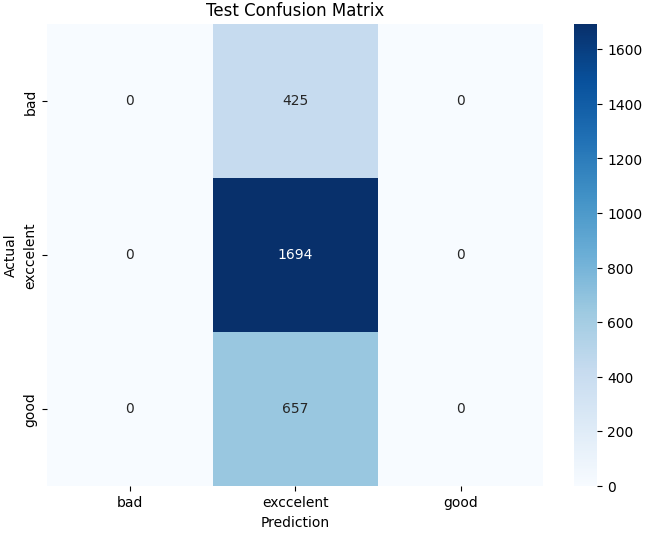
\includegraphics[width=70mm]{Naive_bayse.png}
\caption{Naive Bayesの混合行列}
\label{Naivebayse.png}
\end{center}
\end{figure}

\begin{figure}[H]
\begin{center}
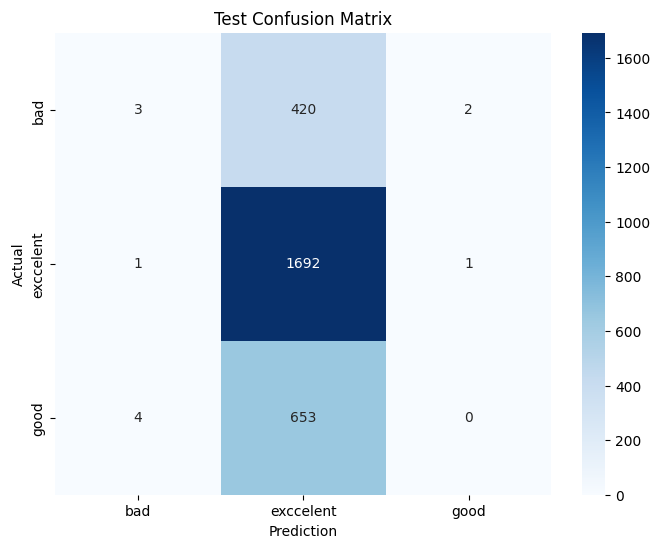
\includegraphics[width=70mm]{SVM.png}
\caption{SVMの混合行列}
\label{SVM.png}
\end{center}
\end{figure}

\begin{figure}[H]
\begin{center}
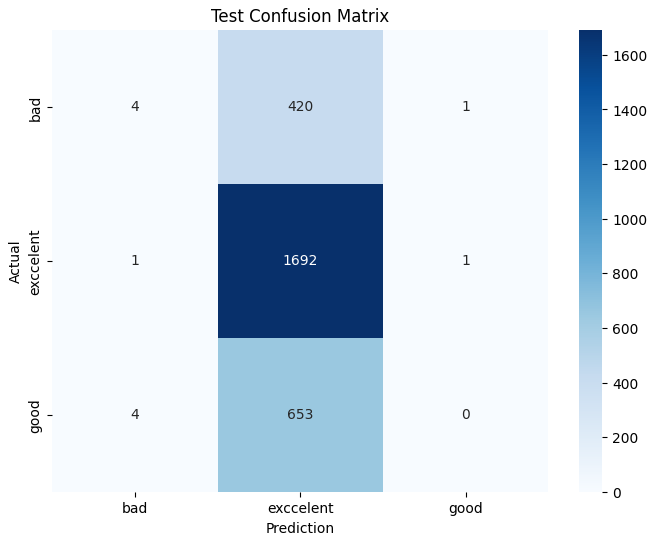
\includegraphics[width=70mm]{DecisionTree.png}
\caption{Decision Treeの混合行列}
\label{DecisionTree.png}
\end{center}
\end{figure}

\begin{figure}[H]
\begin{center}
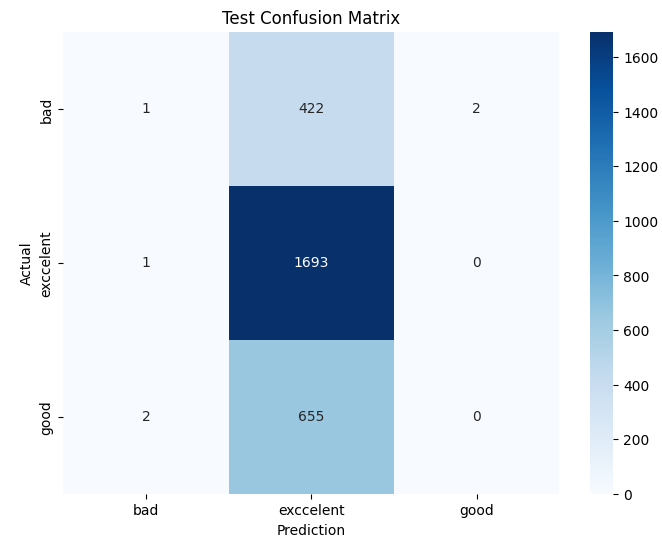
\includegraphics[width=70mm]{LogisticRegression.png}
\caption{Logistic Regressionの混合行列}
\label{LogisticRegression.png}
\end{center}
\end{figure}

 混合行列からわかるようにexccelentの分類はうまく行えているが,good,badともにexccelentに分類されていてうまく分類できていないことがわかる.



% \newpage
% \thispagestyle{nohead}
% \end{titlepage}


\section{結論と今後の課題}
\label{conclusions}
\subsection{結論と考察}

 今回の結果からアルゴリズムはDistilBERTが一番精度が高いことが分かったが,その反面実行時間に難があり,バッチサイズやデータを少数にしても約10分ほどの実行時間を要することが分かった.しかし,同じアルゴリズムやシステムを使ってレビュー文の評価分類やそのほかの分類も行いたいと考えている.
 
 実行時間を考えると明らかにDistilBERT以外のアルゴリズムを使った方が精度は低いがいいだろう.しかし,レビューの分類において精度は大切であるので,DisitlBERTを使用することになるだろう.

 精度の問題に関しても,テストスコアが低すぎるという問題が発生している.原因の一つとしてスパムレビューの存在が考えられる.以前もDistilBERTに学習させる前に分かち書きや形態素解析を行いストップワードや記号の除去をしていたが,それでは記号だけが取り除かれた変な文章のみが残り,それが精度の低下に関係していると考えられる.そのためスパムレビューだと判断しそのレビューを学習データから外すという操作が必要であると考える.
 
 また,外国人からのレビューも精度を低下させる原因となってしまうため,本研究ではスパムメールとして扱うことにする.
 スパムレビューの例としてTable\ref{spam}のようなレビューがある.
 \begin{table}[H]\centering
  \caption{スパムレビュー例}
  \label{spam}
\begin{tabular}{|l|l|} \hline
   type & レビュー文   \\ \hline
   exccelent& 多謝。   \\\hline
   good &  ・カレーは。 \\ 
   good & Wに利用しました。\\
   good & って思ってます。 \\
   good & と考えさせられました。 \\ \hline
   bad  & )のが残念でした。 \\ \hline
\end{tabular}
\end{table}
 今回考察するにあたってスパムレビューの大多数がgoodのであるが,実際はexccelentに分類されていた.

 今後研究するにあたり,スパムレビューの分類およびその数についても発表し,学習データの各種類ごとにスパムのレビューがどのくらいあるのかを調べていきたいと思う.

 また,もう一つ精度が下がった原因として考えられるものは過学習である.今回用意したデータのタイプの数はFigure\ref{data_type}に示しているが,全データ数5551データに対し,exccelentのデータが3405件と半数以上のデータがexccelentであるということがわかる.そこでNaivebayseでの誤分類されたデータをランダムで表示させたものをTable\ref{matigae}に示す.

\begin{table}[htbp]\centering
  \caption{誤分類された文章}
  \label{matigae}
\begin{tabular}{|l|l|l|} \hline
   答え & 予想 & 文章  \\ \hline
   good & exccelent &  改善が必要だと思うます \\
   good & exccelent & また利用するたいとは思うます 。\\
   good & exccelent & まず驚いたのはフロアが物音ひとつせず\\
        &            &自分の整理の音さえ気にする程でした。\\
   bad & exccelent  & 大 浴場 が ない 。\\
   bad & exccelent  &トイレ が 狭い 。\\
   bad & exccelent & 3オーシャンビューであるが前回は綺麗\\
       &            &に晴れていてエーゲ海のような絶景で\\
       &            &あったが今回は少しもやがかかっていて\\
       &            &残念であった。\\ \hline
\end{tabular}
\end{table}

Table\ref{matigae}からわかることは,good,badのレビューがexccelentに分類されてしまっているということである.
 
\subsection{今後の課題}
 今後については現在作成しているレビュー文の分類は宿泊施設の評価を分類しているが次は季節について分類を行っていきたいと考えている.
 
 今回行ったレビュー文の分類の結論とシステムの構築から今後次のようなことに取り組んでいきたいと考えている.
\begin{enumerate}
  \item DistilBERTの精度向上(スパムレビューの排除)
  \item 教師あり学習のためテストデータ(レビュー文)の季節分類分けを行う
  \item レコメンドシステムを使った推薦システムの開発
  \item システムを完成させる
\end{enumerate}

 1つ目に今回の結果からDistilBERTを使用しても精度が低くなってしまうという結果が出たが,スパムレビューを除去することによって精度を上げつつ過学習であるかexccelentのレビューを少なくすることによって調べていきたいと考えている.

 2つ目に今回使用した学習データはタイプ分けとして評価のタイプ分けのみしか行われていない.今後季節別にレビュー文を分類するにあたって学習データの分類を行わなければならない.
 
 3つ目に今回行った評価別に分けるものと季節別に分けるもの,そのほかにもユーザーデータや観光地情報などを使い,レコメンドシステムを使った推薦システムの開発を行う予定である.
 
 最後に観光システム全体としてWeb・SNSからデータを収集することや,ユーザーに推薦するためのWebページが完成していないためそちらを完成させるとともに,推薦システムの要素として評価の情報追加できるようにしたいと考えている.
\bibliographystyle{jplain}
%\bibliography{bibliography.bib}


% \begin{thebibliography}{}
% \bibitem{solomon93}Robert C. Solomon. 1993. \textit{The Passions: Emotions and the Meaning of Life}, Hackett Publishing.
% \bibitem{beijer02}Fabian Beijer. 2002. The syntax and pragmatics of exclamations and other expressive/emotional utterances. \textit{Working Papers in Linguistics 2}, The Dept. of English in Lund. 
% \bibitem{ono02}Hajime Ono. 2002. \textit{An emphatic particle DA and exclamatory sentences in Japanese}. University of California, Irvine.
% \bibitem{kamei96}Takashi Kamei, Rokuro Kouno and Eiichi Chino (eds.). 1996. \textit{The Sanseido Encyclopedia of Linguistics}, Vol. VI, Sanseido.
% \bibitem{crystal89}David Crystal. 1989. \textit{The Cambridge Encyclopedia of Language}. Cambridge University Press. 
% \end{thebibliography}
 \begin{thebibliography}{99}
  \bibitem{hokkaidou_data} 
  国土交通省 北海道運輸局,北海道の観光基礎データ,
\url{https://wwwtb.mlit.go.jp/hokkaido/content/000284820.pdf},2024年7月11日閲覧

 \bibitem{baitai_data}
 日本交通公社,国内旅行におけるSNS,写真に対する意識/実態,
\url{https://www.jtb.or.jp/research/statistics-tourist-sns-pictures2022},2024年7月11日閲覧


 \bibitem{review_data}
 「じゃらんクチコミデータ」,株式会社リクルート,
\url{https://github.com/megagonlabs/jrte-corpus/blob/master/data/pn.tsv}

\bibitem{ronbun2}
林部 祐太,知識の整理のための根拠付き自然文間含意関係コーパスの構築,
\url{https://www.anlp.jp/proceedings/annual_meeting/2020/pdf_dir/P4-9.pdf}

\bibitem{slothlib}
Slothlib,
\url{http://svn.sourceforge.jp/svnroot/slothlib/
CSharp/Version1/SlothLib/NLP/Filter/StopWord/word/Japanese.txt}

\bibitem{Naivebayse}
Naive Bayes,
\url{https://docs.oracle.com/cd/E15817_01/
datamine.111/e05704/algo_nb.html}

\bibitem{SVM}
1.4. Support Vector Machines,
\url{https://scikit-learn.org/stable/modules/svm.html}


\bibitem{Decision Tree}
1.10. Decision Trees,
\url{https://scikit-learn.org/stable/modules/tree.html}


\bibitem{Logistic Regression}
LogisticRegression — scikit-learn 1.5.1 documentation, 
\url{https://scikit-learn.org/stable/modules/generated/sklearn.linear_model.LogisticRegression.html}

\bibitem{BERT}
BERT: Pre-training of Deep Bidirectional Transformers for Language Understanding,Jacob Devlin, Ming-Wei Chang, Kenton Lee, Kristina Toutanova,
\url{https://arxiv.org/abs/1810.04805}

\bibitem{DistilBERT}
DistilBERT, a distilled version of BERT: smaller, faster, cheaper and lighter ,
Victor Sanh, Lysandre Debut, Julien Chaumond, Thomas Wolf,
\url{https://arxiv.org/abs/1910.01108}

\end{thebibliography}


\end{document}